\xchapter{Análise da complexidade estrutural das ferramentas}{}

%4 analise das complexidade das ferramentas + metodologia + resultados
%  * analizo
% apresentar parte da antiga metologia aqui, apresentar alguns resultados

\section{Coleta de dados}

Coletamos para cada ferramenta selecionada suas métricas de código-fonte através
da execução da ferramenta {\it analizo metrics}, esta coleta foi automatizada pelo
script {\it analyze-all-projects} escrito durante este estudo disponível no repositório
git desta pesquisa\footnote{http://github.com/joenio/dissertacao-ufba-2016/blob/master/dataset/analyze-all-projects}.

\section{Análise de dados} \label{analise}

Os dados coletados incluem métricas de código-fonte para cada módulo/classe de
cada ferramenta selecionada, tanto da indústria quanto da academia. As
métricas a serem analisadas e interpretadas são as métricas descritas na Seção
\ref{metricas-de-codigo}.

A linguagem R \cite{Ihaka1996}, uma linguagem de programação para cálculos
estatísticos e gráficos, será utilizada para manipulação de dados, criação de
tabelas e plotagem de gráficos. Todos os cálculos em linguagem R utilizados
neste trabalho estão disponíveis
em nosso repositório\footnote{http://github.com/joenio/dissertacao-ufba-2016/blob/master/qualificacao.R}.

\subsection{Distribuição dos valores das métricas}

Iremos calcular os percentis de cada métrica para cada ferramenta a partir dos
valores das métricas dos seus módulos, um percentil é a centésima parte dos
dados ordenados de forma crescente, iremos calcular os percentis 1, 5, 10, 25,
50, 75, 90, 95 e 99, e dentre eles iremos discutir os resultados em função dos
percentis 75, 90 e 95, assim como feito por \citeonline{Meirelles2013},
correspondendo a valores muito frequentes, frequentes e pouco frequentes,
respectivamente.

Esta discussão irá nos fornecer como resultado intervalos de referência para
métricas de código-fonte neste domínio de aplicação, estes intervalos serão
definidos a partir da interpretação manual dos percentis e serão analisados
usando modelos de regressão a fim de serem compreendidos e validados, uma
comparação com intervalos encontrados nos trabalhos relacionados (seção
\ref{trabalhos-relacionados}) também será realizada com objetivo de reforçar
estes valores.

...

\section{Analizo} \label{analizo}

Esta seção apresenta a ferramenta Analizo utilizada neste estudo para
coletar métricas de código-fonte das ferramentas utilizadas como objeto de
estudo.

Analizo é um conjunto de ferramentas para análise de código-fonte e
visualização, desenvolvido tendo como requisitos suportar múltiplas linguagens
de programação, ser software livre, ser extensível e que seja capaz de lidar
com código-fonte não mais compilável.

Este último requisito permite analisar código-fonte com erros de sintaxe, com
referências a bibliotecas não mais disponíveis, ou que usem bibliotecas com
mudanças de API em versões mais recentes. Isto é importante especialmente ao
analisar código-fonte legado em estudos sobre evolução de software.

Ela será a ferramenta utilizada por nós durante este estudo para análise do
código-fonte das ferramentas selecionadas, a decisão pela ferramenta Analizo
se deu por conta dela ser também a escolha utilizada nos trabalhos
relacionados (seção \ref{trabalhos-relacionados}) onde estamos nos apoiando,
além disso, Analizo também tem sido utilizada em diversos estudos
desenvolvidos em nosso grupo de pesquisa (seção \ref{trabalhos-analizo}).

A seleção de ferramentas a serem estudadas neste trabalho de pesquisa tomará
como um dos critérios de escolha as linguagens de programação suportadas pelo
Analizo, ou seja, apenas ferramentas escritas em C, C++ ou Java farão parte do
nosso estudo.

Analizo é uma ferramenta mantida constantemente, com desenvolvedores ativos, e
atualizações frequentes, sua última versão 1.19.1 foi lançada (no escopo deste
trabalho) em 01 de Setembro de 2016 e será a versão utilizada neste estudo.

\subsection{Arquitetura}

A arquitetura do Analizo é apresentada na Figura \ref{arquitetura-analizo}
através de uma representação do tipo {\it Layered Style} \cite{Clements2002},
onde cada camada no diagrama usa apenas os serviços oferecidos pela camada
diretamente abaixo dela.

\begin{figure}[h]
\center
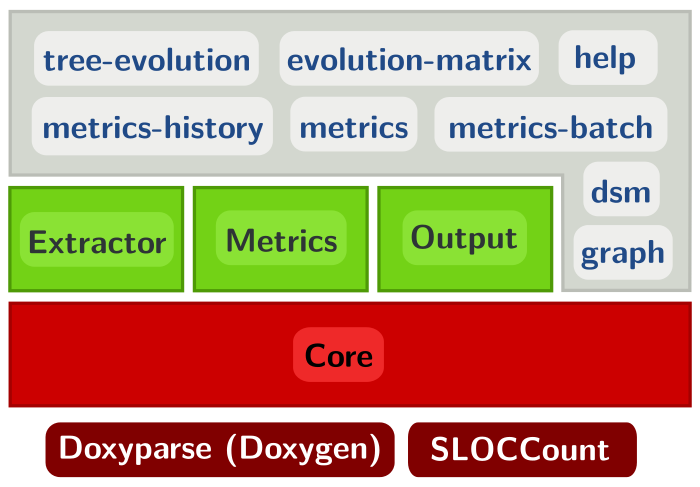
\includegraphics[scale=0.3]{imagens/analizo-architecture.png}
\caption{Arquitetura do Analizo, usando Layered Style \cite{Clements2002}}
\label{arquitetura-analizo}
\end{figure}

O {\it Core} contém as estruturas de dados usadas para armazenar informações a
respeito do código-fonte sendo analisado, como a lista de módulos\footnote{o
conceito ``módulo'' é usado como um termo abrangente para designar diferentes
tipos de estruturas usados em desenvolvimento de software, como classes e
arquivos fonte C}, elementos dentro de cada módulo (atributos, variáveis,
métodos, funções), informações de dependência (chamada, herança, etc). Esta
camada implementa a maior parte da lógica de negócio do Analizo, e não depende
de nenhuma outra camada.

A camada {\it Extractor} lida com as informaçoes de código-fonte obtidas pelas
diferentes estratégias implementadas no Analizo. Os extratores obtém
informações do código-fonte e armazenam em estruturas de dados da camada {\it
Core}. Adicionar um novo extrator requer apenas a criação de uma nova subclasse
que faça interface com uma ferramenta externa ou que ela própria realize análise
de código-fonte. Atualmente existem dois extratores, ambos fazem interface
com ferramentas externas de análise estática de código-fonte:

\begin{itemize}

  \item {\it Analizo::Extractor::Doxyparse} é uma interface para o Doxyparse,
  um parser de código-fonte para C, C++ e Java desenvolvida por nosso grupo de
  pesquisa\cite{Costa2009}. Doxyparse é baseado no
  Doxygen\footnote{doxygen.org}, um sistema de documentação multi-linguagem.

  \item {\it Analizo::Extractor::Sloccount} é uma interface para o
  Sloccount\footnote{dwheeler.com/sloccount} desenvolvido por David A. Wheeler,
  uma ferramenta que calcula o número efetivo de linhas de código.

\end{itemize}

As outras camadas intermediárias são {\it Metrics} e {\it Output}. A camada
{\it Metrics} processa as estruturas de dados do {\it Core} para calcular
métricas, até o momento Analizo suporta um conjunto razoável de métricas
(listadas na Seção \ref{metricas}), uma representação desta camada pode ser
vista no diagrama da Figura \ref{arquitetura-metrics-analizo}. A camada {\it
Output} é responsável por lidar com diferentes formatos de arquivos.
Atualmente, apenas o formato DOT é implementado no Analizo para representar
grafo de dependencia, adicionar novos formatos é simplesmente adicionar novas
classes nesta camada.

\begin{figure}[H]
\center
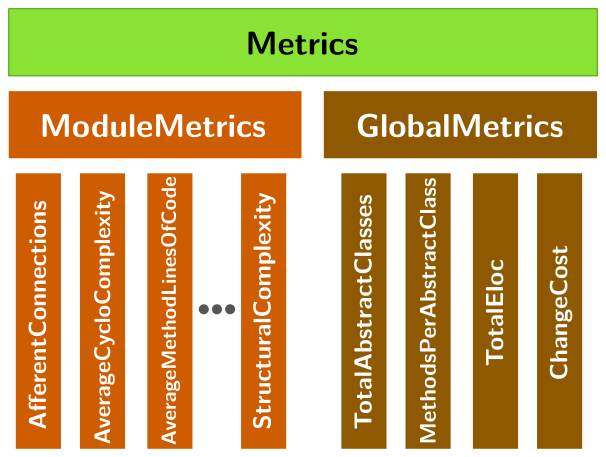
\includegraphics[scale=0.4]{imagens/analizo-metrics-architecture.png}
\caption{Arquitetura do módulo metrics em detalhe, usando Layered Style \cite{Clements2002}}
\label{arquitetura-metrics-analizo}
\end{figure}

A camada {\it Tools} fornece um conjunto de ferramentas de linha de comando que
constituem a interface do analizo, tanto para usuários finais quanto para
aplicações de mais alto nível. Estas ferramentas usam serviços providos pelas
outras camadas: eles instanciam as estruturas de dados do {\it Core},
inicializam um ou mais extratores, opcionalmente executam o processador de
métricas, instanciam um módulo de formato de saída, e gerencia todos eles para
prover o resultado desejado. A maioria das funcionalidades descritas na Seção
\ref{funcionalidades} são implementadas na camada {\it Tools} do Analizo.

Estas ferramentas são pensadas na filosofia UNIX: fazem uma tarefa
especializada e geram uma saída que pode ser utilizada como entrada para outras
ferramentas, seja para o próprio Analizo ou para ferramentas externas. Algumas das
ferramentas implementadas no Analizo são feitas consumindo saída gerada por
outra ferramenta ao invés de manipular explicitamente os internos do Analizo,
algumas outras são desenhadas para prover saída em formato específico para
aplicacoes externas, como por exemplo programas para desenho de grafos ou
visualização de dados.

\subsection{Funcionalidades}\label{funcionalidades}

\subsubsection{Análise de código-fonte multi-linguagem}

Atualmente Analizo suporta análise de código-fonte escrito em C, C++ e Java.
Entretanto, pode ser facilmente estendido para suportar outras linguagens pois
pode potencialmente suportar as inúmeras outras linguagens suportadas pelo Doxygen.

\subsubsection{Métricas}\label{metricas}

O Analizo suporta tanto métricas em nível de projeto, que é calculada para todo o projeto,
quanto métricas em nível de módulos, que é calculado individualmente para cada módulo.
No nível de projeto, Analizo também provê estatística descritiva básica para cada métrica em
nível de módulo: soma, média, mediana, moda, desvio padrão, variância, skewness e kurtosis da
distribuição, valores mínimo e maximo. As seguintes métricas são suportadas até o momento:

\begin{itemize}

  \item Métricas em nível de projeto: Change Cost, Total Abstract Classes,
  Total Coupling Factor, Total Effective Lines of Code, Total Lines of Code,
  Methods per Abstract Class, Total Number of Modules, Total number of modules
  with at least one defined attributes, Total number of modules with at least
  one defined method, Total Number of Methods.

  \item Métricas em nível de módulo: Afferent Connections per Class, Average
  Cyclomatic Complexity per Method, Average Method Lines of Code, Argument with
  'nonnull' attribute passed null, Average Number of Parameters per Method,
  Allocator sizeof operand mismatch, Assigned value is garbage or undefined,
  Bad deallocator, Bad free, Coupling Between Objects, Dead assignment,
  Divisions by zero, Double free, Depth of Inheritance Tree, Dereference of
  null pointer, Dereference of undefined pointer value, Potential buffer
  overflow in call to 'gets', Lack of Cohesion of Methods, Lines of Code,
  Memory leak, Max Method LOC, Number of Attributes, Number of Children, Number
  of Methods, Number of Public Attributes, Number of Public Methods,
  Out-of-bound array access, Offset free, Potential insecure temporary file in
  call 'mktemp', Response for a Class, Result of operation is garbage or
  undefined, Return of stack variable address, Stack address stored into global
  variable, Structural Complexity, Undefined allocation of 0 bytes,
  Use-after-free, Uninitialized argument value.

\end{itemize}

É possível especificar que certos diretórios dentro do projeto não devem ser
analisados, de forma que o Analizo ignore tais arquivos durante a análise e o
cálculo de métricas.

\subsubsection{Processamento em lote}\label{lote}

A maioria dos estudos quantitativos em Engenharia de Software envolve aquisição
de métricas de código-fonte de um grande número de projetos, processar cada
projeto individualmente é pouco prático, passível de erros e difícil de
repetir. Analizo pode processar multiplos projetos em lote e produzir arquivo
de dados CSV com métricas de cada projeto, bem como um resumo com as métricas
em nível de projeto de todos os projetos. Estes arquivos de dados podem ser
facilmente importados em ferramentas de estatística ou planilhas para análise
futura. Esta capacidade de processar em lote pode também ser utilizada para
analisar várias versões de um mesmo projeto, especialmente útil em estudos
sobre evolução de software.

Este processamento em lote pode se beneficiar de processamento paralelo dando
mais agilidade e na análise e reduzindo o tempo total de processamento.  A
saída pode ser também escrita diretamente em um banco de dados relacional ao
invés de gerar arquivos CSV. Outro recurso voltado à performance é um sistema
de cache para as informações previamente calculadas, evitando repetição de
processamento.

\subsubsection{Histórico de métricas}

Algumas vezes pesquisadores precisam processar o histórico de projetos de
software de uma forma mais escalável. Analizo pode processar repositórios de
controle de versão e prover arquivo de dados CSV com valores de métricas para
cada revisão onde o código-fonte foi alterado no projeto, ou pode também gravar
os valores diretamente num banco de dados ao invés de usar arquivos CSV. Repositórios Git e
Subversion são suportados diretamente, repositórios CVS devem ser convertidos
para Git de forma manual.

\subsubsection{Grafo de dependência}

Analizo pode gerar saída com informações sobre dependência entre as entidades
do projeto em um formato adequado para processamento por ferramentas de
renderização de grafos do Graphviz\footnote{graphviz.org}. A Figura
\ref{sample-graph} apresenta um exemplo de grafo desenhado pela ferramenta {\it
dot} do Graphviz a partir da saída gerada pelo Analizo {\it graph}.

\begin{figure}[h]
\center
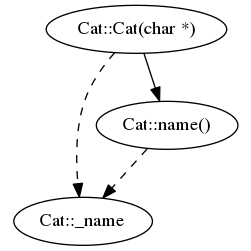
\includegraphics[scale=0.4]{imagens/sample-graph.png}
\caption{Exemplo de grafo de dependência}
\label{sample-graph}
\end{figure}

\subsubsection{Matriz de evolução}

Outra funcionalidade útil do Analizo é a visualização de matrizes de evolução
\cite{Lanza2001}. Ao processar cada release de um projeto (ver Seção
\ref{lote}), o usuário pode solicitar a criação de uma matrix de evolução a
partir de arquivos de dados individuais. A Figura \ref{sample-evolution-matrix}
apresenta um exemplo de uma matrix produzida pelo Analizo.

\begin{figure}[h]
\center
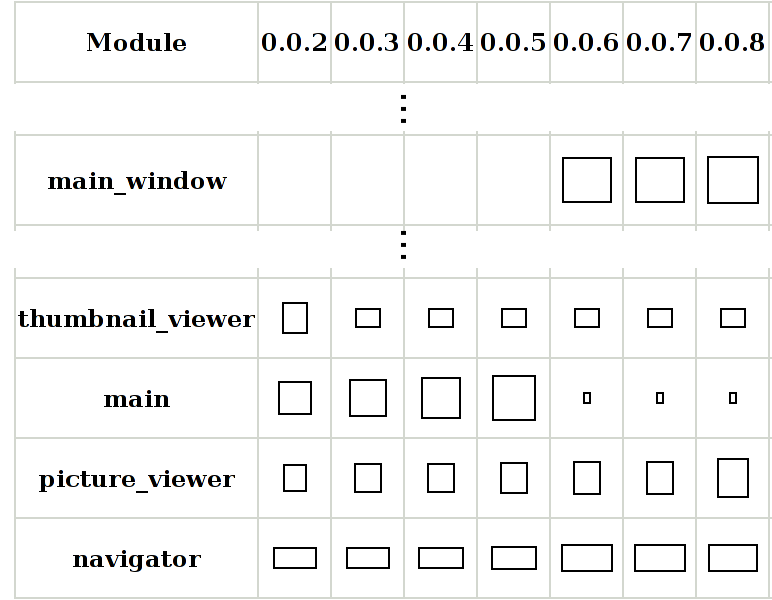
\includegraphics[scale=0.2]{imagens/sample-evolution-matrix.png}
\caption{Exemplo de matrix de evolução}
\label{sample-evolution-matrix}
\end{figure}

\subsubsection{Matriz de estrutura de projeto}

Uma funcionalidade recente do Analizo é a representação visual do
relacionamento entre os módulos do projeto em forma de uma Matriz de estrutura
de projeto ({\it Design Structure Matrix}) \cite{Maccormack2006}, uma DSM é a
representação de um grafo de dependência em forma de uma matriz quadrada. Um
exemplo gerado pelo Analizo pode ser visto na Figura \ref{sample-dsm}.

\begin{figure}[h]
\center
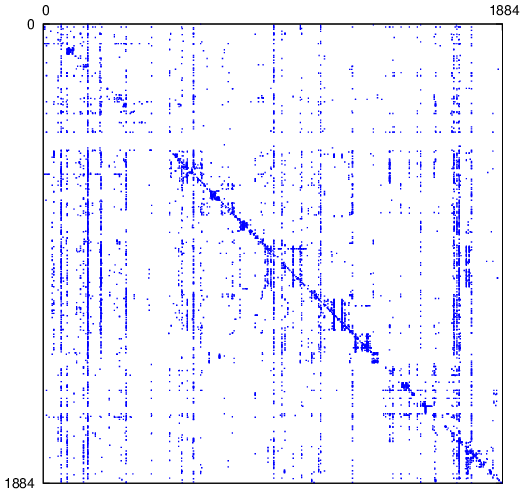
\includegraphics[scale=0.3]{imagens/sample-dsm.png}
\caption{Exemplo de matrix de estrutura de projeto}
\label{sample-dsm}
\end{figure}

\subsection{Uso em trabalhos de pesquisa}
\label{trabalhos-analizo}

Analizo tem sido extensivamente usada por nosso grupo de pesquisa em diversos
estudos:

\begin{itemize}

  \item \cite{Amaral2009} usou o grafo de dependencia gerado pelo Analizo para
  gerar uma matriz de evolução em um estudo de caso com o projeto VLC.

  \item \cite{Costa2009} fez uma comparação entre diferentes estratégias para
  extração de informação de dependencias entre módulos do código-fonte,
  resultando no desenvolvimento do Doxyparse - o extrator baseado no Doxygen do
  Analizo.

  \item \cite{Terceiro2009} usou métricas em um estudo exploratório sobre a
  evolução da complexidade estrutural em projetos de software livre escritos em
  C.

  \item \cite{Morais2009} usou a ferramenta de métricas do Analizo como backend
  para o Kalibro, um software para avaliação e observação de métricas de código-fonte.
  
  \item \cite{Terceiro2010} usou o processamento de histórico de métricas para
  realizar um estudo exploratório sobre a evolução da complexidade estrutural em
  7 projetos de servidor web de diferentes tamanhos.

  \item \cite{Meirelles2010} usou o processamento em lote do Analizo para
  processas o código-fonte de mais de 6000 projetos de software livre do
  repositório Sourceforge.net.

  \item \cite{Meirelles2011} usou o Analizo em um estudo sobre impacto de
  métricas de código-fonte na atratividade de projetos de softwares livres.

  \item \cite{Terceiro2012Understanding} usou o Analizo para investigar fatores
  que influenciam na evolução da complexidade estrutural em projetos de software
  livres.

  \item \cite{Silva2012} usou o Analizo para minerar 16000 revisões de
  repositórios de projetos de software para investigar o potencial de uma nova
  métrica chamada Lack of Concern-based Cohesion.

  \item \cite{Ronaldo2015} utilizou o Analizo para extrair métricas de
  código-fonte de 14 versões do sistema Android e estudar a evoluçao da API e
  seus aplicativos.

\end{itemize}

A maioria destes trabalhos contribuíram com melhorias para o Analizo, fazendo
dele ainda mais apropriado para pesquisas envolvendo análise de código-fonte.

\subsection{Considerações finais}

Apresentamos o Analizo, um conjunto de ferramentas para análise e
visualização de código-fonte com suporte a C, C++ e Java. Analizo é útil tanto
para pesquisadores trabalhando com análise de código-fonte quanto para
profissionais que precisam analisar seus projetos em busca de
potenciais problemas ou melhorias.

Analizo é software livre, licenciado sob a GNU General Public License versão 3.
Seu código-fonte, bem como pacotes binários, manuais e tutoriais podem ser
obtidos em http://analizo.org. Todas as ferramentas são auto-documentadas e
podem ser consultadas como páginas de manual UNIX. Analizo é escrito em Perl.
